\newcommand{\EstimatorResults}{
\begin{tabular}{lrrr}
\toprule
Estimator & MAE [95\% seed CI] & Bias & Cal. interval coverage \\ \midrule
CAL & 0.0913 [0.0901, 0.0924] & +0.0381 & 0.632 \\
RAW & 0.0908 [0.0895, 0.0921] & +0.0409 & 0.632 \\
ATC & 0.1201 [0.1162, 0.1238] & +0.0469 & 0.632 \\
CONSTANT & 0.0931 [0.0922, 0.0941] & +0.0299 & 0.632 \\
\bottomrule
\end{tabular}
}
\newcommand{\DetectorResults}{
\begin{tabular}{llrrr}
\toprule
Regime & Detector & False alarm rate & Detection rate & Mean lag (batches) \\ \midrule
M0 stationary & KS/PCA & 0.048 & 0.978 & 22.25 \\
M0 stationary & Pairwise correlation & 0.066 & 0.889 & 15.75 \\
M1 abrupt nuisance & KS/PCA & 0.048 & 1.000 & 0.00 \\
M1 abrupt nuisance & Pairwise correlation & 0.066 & 0.889 & 15.75 \\
M2 gradual predictive & KS/PCA & 0.048 & 1.000 & 2.27 \\
M2 gradual predictive & Pairwise correlation & 0.066 & 0.889 & 15.75 \\
M3 incremental repeated small & KS/PCA & 0.048 & 1.000 & 0.11 \\
M3 incremental repeated small & Pairwise correlation & 0.066 & 0.889 & 15.75 \\
M4 abrupt conditional reversal & KS/PCA & 0.048 & 0.978 & 22.25 \\
M4 abrupt conditional reversal & Pairwise correlation & 0.066 & 0.889 & 15.75 \\
M5 recurrent conditional reversal & KS/PCA & 0.048 & 0.978 & 22.25 \\
M5 recurrent conditional reversal & Pairwise correlation & 0.066 & 0.889 & 15.75 \\
M6 dependence marginals preserved & KS/PCA & 0.048 & 0.978 & 11.40 \\
M6 dependence marginals preserved & Pairwise correlation & 0.066 & 1.000 & 0.03 \\
M7 out of support & KS/PCA & 0.048 & 1.000 & 0.00 \\
M7 out of support & Pairwise correlation & 0.066 & 0.889 & 15.75 \\
\bottomrule
\end{tabular}
}
\newcommand{\DelayResults}{
\begin{tabular}{rrrrr}
\toprule
Delay & Age at release & Accuracy after release & Verified harm fraction & Verified batches \\ \midrule
0 & 0 & 0.578 & 0.233 & 11,520 \\
5 & 5 & 0.578 & 0.233 & 11,520 \\
20 & 20 & 0.578 & 0.233 & 11,520 \\
100 & 100 & 0.578 & 0.233 & 11,520 \\
\bottomrule
\end{tabular}
}
\newcommand{\ReleasedErrorResults}{
\begin{tabular}{rrrrr}
\toprule
Delay & Stationary false alarm & Drift detected by input end & Drift detected after drain & Mean lag (source batches) \\ \midrule
0 & 0.000 & 0.487 & 0.487 & 5.66 \\
5 & 0.000 & 0.487 & 0.487 & 5.66 \\
20 & 0.000 & 0.487 & 0.487 & 5.66 \\
100 & 0.000 & 0.000 & 0.487 & 5.66 \\
\bottomrule
\end{tabular}
}
\newcommand{\PairedResults}{
\begin{tabular}{lrrr}
\toprule
Comparator & Mean paired $\Delta$MAE & Holm $q<.05$ strata & Strata \\ \midrule
CAL $-$ RAW & +0.0001 & 37 & 120 \\
CAL $-$ ATC & -0.0257 & 99 & 120 \\
CAL $-$ CONSTANT & -0.0019 & 12 & 120 \\
\bottomrule
\end{tabular}
}
\newcommand{\DimensionSensitivity}{\subsection{Feature-dimensionality sensitivity}This separate locked extension contains 1,440 task--mechanism--seed--dimension cells and repeats the estimator comparison at 32 and 128 features; the primary eight-feature result is included for reference. Seed-bootstrap intervals resample complete seed blocks and describe Monte Carlo variability conditional on these synthetic laws.\par{}Descriptively, calibrated-estimator MAE was d=8: 0.0913, d=32: 0.0841, d=128: 0.0719; raw Average Confidence was d=8: 0.0908, d=32: 0.0888, d=128: 0.0959. The synthetic feature space and signal-to-noise ratio change with dimension, so this is a sensitivity of the declared generator family, not an isolated causal test of dimensionality or evidence of a universal trend.\par{}\begin{table}[htbp]\centering\small\begin{tabular}{lrrr}
\toprule
Features & Estimator & Mean seed MAE & 95\% seed-bootstrap interval \\ \midrule
8 & CAL & 0.0913 & [0.0902, 0.0925] \\
32 & CAL & 0.0841 & [0.0831, 0.0851] \\
128 & CAL & 0.0719 & [0.0709, 0.0729] \\
8 & RAW & 0.0908 & [0.0894, 0.0921] \\
32 & RAW & 0.0888 & [0.0876, 0.0901] \\
128 & RAW & 0.0959 & [0.0946, 0.0972] \\
8 & ATC & 0.1201 & [0.1162, 0.1238] \\
32 & ATC & 0.1064 & [0.1035, 0.1096] \\
128 & ATC & 0.0838 & [0.0827, 0.0850] \\
8 & CONSTANT & 0.0931 & [0.0922, 0.0940] \\
32 & CONSTANT & 0.0880 & [0.0870, 0.0890] \\
128 & CONSTANT & 0.0767 & [0.0756, 0.0779] \\
\bottomrule
\end{tabular}\caption{Accuracy-estimation error by feature dimension in the sensitivity run.}\end{table}\begin{figure}[htbp]\centering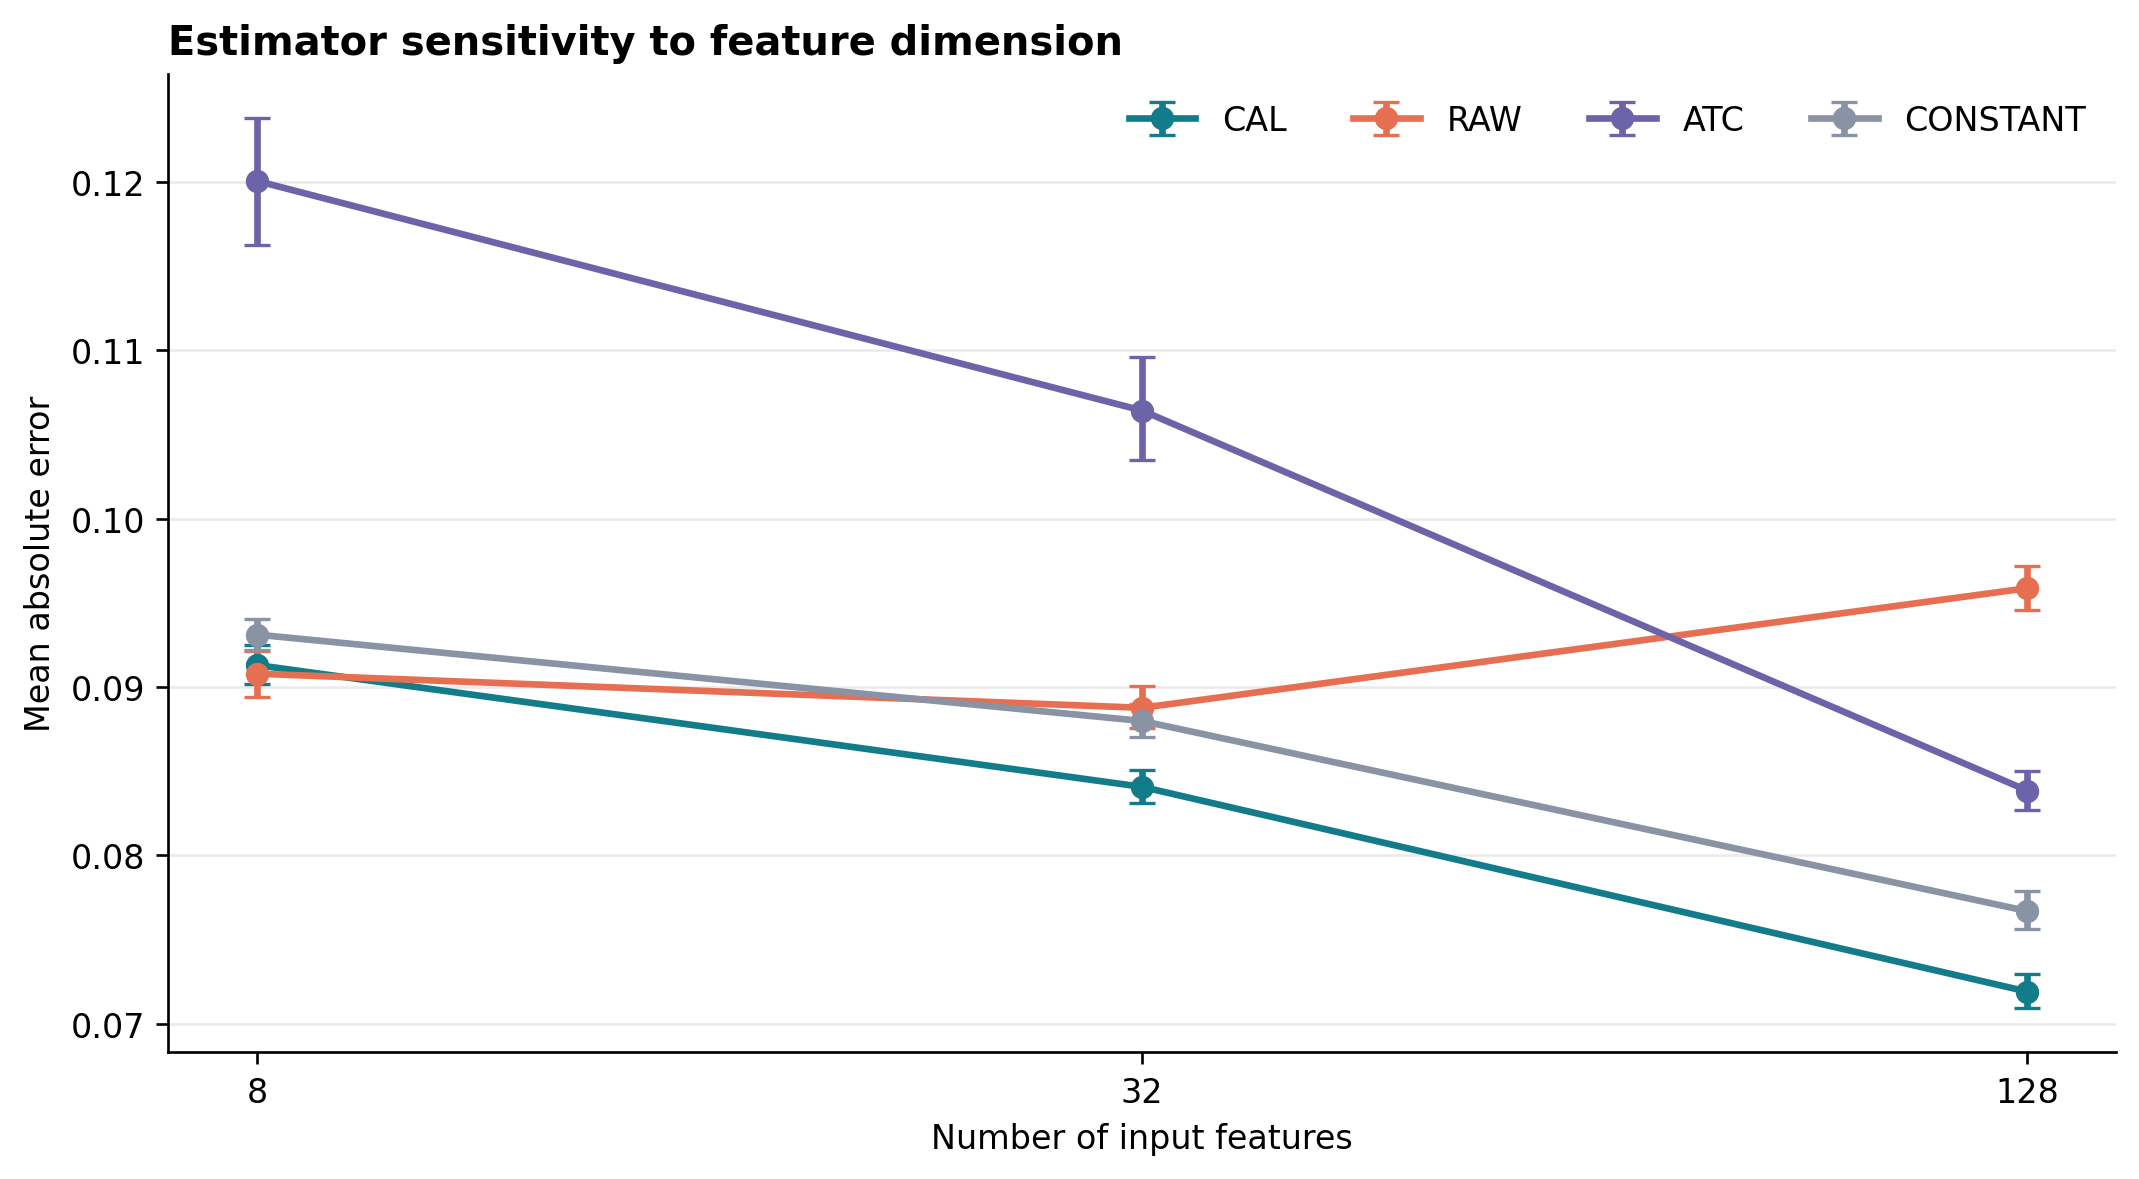
\includegraphics[width=.88\linewidth]{figures/fig05_dimension_sensitivity.png}\caption{Seed-level mean absolute estimation error by feature dimension. Error bars are 95\% seed-bootstrap intervals.}\end{figure}}
